%%%%%%%%%%%%%%%%%%%%%%%%%%%%% Define Article %%%%%%%%%%%%%%%%%%%%%%%%%%%%%%%%%%
\documentclass{article}
%%%%%%%%%%%%%%%%%%%%%%%%%%%%%%%%%%%%%%%%%%%%%%%%%%%%%%%%%%%%%%%%%%%%%%%%%%%%%%%

%%%%%%%%%%%%%%%%%%%%%%%%%%%%% Using Packages %%%%%%%%%%%%%%%%%%%%%%%%%%%%%%%%%%
\usepackage{geometry}
\usepackage{graphicx}
\usepackage{amssymb}
\usepackage{amsmath}
\usepackage{amsthm}
\usepackage{empheq}
\usepackage{mdframed}
\usepackage{booktabs}
\usepackage{lipsum}
\usepackage{graphicx}
\usepackage{color}
\usepackage{psfrag}
\usepackage{pgfplots}
\usepackage{bm}
\usepackage{hyperref}
\usepackage{subcaption}
\usepackage{longtable}

%%%%%%%%%%%%%%%%%%%%%%%%%%%%%%%%%%%%%%%%%%%%%%%%%%%%%%%%%%%%%%%%%%%%%%%%%%%%%%%

% Other Settings

%%%%%%%%%%%%%%%%%%%%%%%%%% Page Setting %%%%%%%%%%%%%%%%%%%%%%%%%%%%%%%%%%%%%%%
\geometry{a4paper}

%%%%%%%%%%%%%%%%%%%%%%%%%% Define some useful colors %%%%%%%%%%%%%%%%%%%%%%%%%%
\definecolor{ocre}{RGB}{243,102,25}
\definecolor{mygray}{RGB}{243,243,244}
\definecolor{deepGreen}{RGB}{26,111,0}
\definecolor{shallowGreen}{RGB}{235,255,255}
\definecolor{deepBlue}{RGB}{61,124,222}
\definecolor{shallowBlue}{RGB}{235,249,255}
%%%%%%%%%%%%%%%%%%%%%%%%%%%%%%%%%%%%%%%%%%%%%%%%%%%%%%%%%%%%%%%%%%%%%%%%%%%%%%%

%%%%%%%%%%%%%%%%%%%%%%%%%% Define an orangebox command %%%%%%%%%%%%%%%%%%%%%%%%
\newcommand\orangebox[1]{\fcolorbox{ocre}{mygray}{\hspace{1em}#1\hspace{1em}}}
%%%%%%%%%%%%%%%%%%%%%%%%%%%%%%%%%%%%%%%%%%%%%%%%%%%%%%%%%%%%%%%%%%%%%%%%%%%%%%%

%%%%%%%%%%%%%%%%%%%%%%%%%%%% English Environments %%%%%%%%%%%%%%%%%%%%%%%%%%%%%
\newtheoremstyle{mytheoremstyle}{3pt}{3pt}{\normalfont}{0cm}{\rmfamily\bfseries}{}{1em}{{\color{black}\thmname{#1}~\thmnumber{#2}}\thmnote{\,--\,#3}}
\newtheoremstyle{myproblemstyle}{3pt}{3pt}{\normalfont}{0cm}{\rmfamily\bfseries}{}{1em}{{\color{black}\thmname{#1}~\thmnumber{#2}}\thmnote{\,--\,#3}}
\theoremstyle{mytheoremstyle}
\newmdtheoremenv[linewidth=1pt,backgroundcolor=shallowGreen,linecolor=deepGreen,leftmargin=0pt,innerleftmargin=20pt,innerrightmargin=20pt,]{theorem}{Theorem}[section]
\theoremstyle{mytheoremstyle}
\newmdtheoremenv[linewidth=1pt,backgroundcolor=shallowBlue,linecolor=deepBlue,leftmargin=0pt,innerleftmargin=20pt,innerrightmargin=20pt,]{definition}{Definition}[section]
\theoremstyle{myproblemstyle}
\newmdtheoremenv[linecolor=black,leftmargin=0pt,innerleftmargin=10pt,innerrightmargin=10pt,]{problem}{Problem}[section]
%%%%%%%%%%%%%%%%%%%%%%%%%%%%%%%%%%%%%%%%%%%%%%%%%%%%%%%%%%%%%%%%%%%%%%%%%%%%%%%

%%%%%%%%%%%%%%%%%%%%%%%%%%%%%%% Plotting Settings %%%%%%%%%%%%%%%%%%%%%%%%%%%%%
\usepgfplotslibrary{colorbrewer}
\pgfplotsset{width=8cm,compat=1.9}
%%%%%%%%%%%%%%%%%%%%%%%%%%%%%%%%%%%%%%%%%%%%%%%%%%%%%%%%%%%%%%%%%%%%%%%%%%%%%%%

%%%%%%%%%%%%%%%%%%%%%%%%%%%%%%% Title & Author %%%%%%%%%%%%%%%%%%%%%%%%%%%%%%%%
\title{Visualización de datos de alta dimesionalidad}
\author{Leonel Guerrero\\ carnet: 18-10638}
%%%%%%%%%%%%%%%%%%%%%%%%%%%%%%%%%%%%%%%%%%%%%%%%%%%%%%%%%%%%%%%%%%%%%%%%%%%%%%%

\begin{document}
\maketitle

\section*{Enunciado}

En esta tarea, usted puede elaborar sus propia implementación de una SOM o usar alguna existente. Recuerde citar la fuente en caso de que use alguna otra implementación y asegúrese de que el algoritmo se corresponde al visto en clase. En el caso de la t-sne puede usar las implementaciones provistas por su autor. La entrega consiste de un informe con los resultados obtenidos.

\begin{enumerate}
  \item Utilice los datos de representación de textos (todos los datos - las 9 categorías) y use la SOM y un t-sne para comparar las visualizaciones obtenidas por estos métodos. Comente sobre el efecto del método de visualización en la información que podemos extraer de esas visualizaciones. Comente ademas en relación con sus entregas previas las implicaciones de las características observadas en relación a la capacidad de que una maquina separe los subconjuntos que se usaron para las tareas del Perceptron, Adeline, MLP y SVM. Concuerdan sus resultados previos con lo que están observando?
\end{enumerate}

\section*{Self Organizing Maps (SOM)}

\subsection*{Descripción de la implementación}

Para la visualización de los datos se utilizo una implementación realizada en python, en la librería sklearn\_som, la cual implementa una SOM utilizando el método de Kohonen, esta librería se puede encontrar en el siguiente enlace: \url{https://pypi.org/project/sklearn-som/}, en la descripción de la librería se puede encontrar la referencia de que la implementación esta basada en el método antes mencionado, la documentación para la utilización de la librería se puede encontrar en \url{https://sklearn-som.readthedocs.io/en/latest/}, en ella se especifica los parámetros que se pueden variar en la implementación de la SOM, los cuales los mas relevantes son la taza de aprendizaje y el parámetro de dispersion de los vecinos, para la visualización de los datos se utilizo la librería matplotlib, la cual permite la visualización de los datos en un plano 2D.
\\

Los parámetros escogidos para la implementación de la SOM fueron los siguientes:

\begin{itemize}
  \item Taza de aprendizaje: 0.1
  \item $\sigma$: 1
  \item Cantidad de épocas: 40
  \item Mallado de la SOM: $10x10$
\end{itemize}

Estos parámetros se escogieron por una pequeña experimentación que se hizo con la librería, al igual que se basaron en los mejores parámetros obtenidos en las tareas previas

\subsection*{Análisis de los resultados}

Se entreno la SOM con el dataset obtenido de los datos de representación de textos científicos, se entreno con las 9 clases contenidas en los 9 archivos, después del entrenamiento se realizo una predicción de cada una de las clases, cada predicción de las clases se representa como un arreglo de longitud 100 ($10x10$), este vector se utilizaron para contar cuantas veces se repetía la activación (neurona ganadora) de una neurona en especifico, para después realizar el coloreamiento del mallado, el coloreamiento se realizo de tal manera que entre mas veces se activara una neurona mas intenso seria el color y entre menos se activara mas negro seria el color de esa neurona, en base a lo descrito previamente se obtuvo la siguiente visualización:

\begin{figure}[!ht]
  \centering
  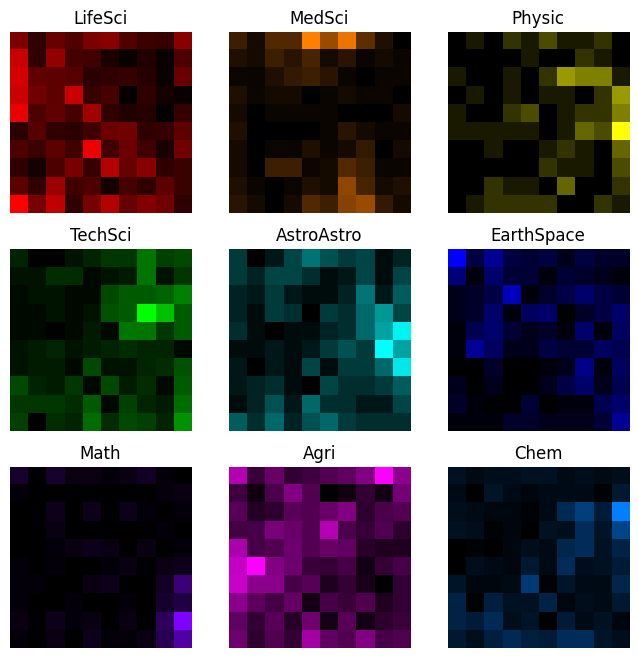
\includegraphics[width=0.7\linewidth]{images/output.png}
  \caption{Visualización de los datos de representación de textos científicos}
  \label{fig:output}
\end{figure}

\newpage

De las visualizaciones obtenidas se pueden obtener un par de conclusiones que se consideran relevantes, la primera es la gran cercanía que poseen las clases de de Physic y AstroAstro, mas aun que las activaciones mas comunes de AstroAstro son justo alrededor de la clase Physic, una información que posee sentido ya que estas ramas poseen bastante similitud. Un hecho similar se repite con la cantidad de cercanía que poseen las clases Math, Physic y Chem (las 3 principales ciencias), información que tiene sentido con la relación real que poseen estas.

De igual forma se puede apreciar la relación menos fuerte que poseen las clases LifeSci y Agri, aunque en ambas se tiene una dispersion de activaciones relativamente elevada, la relación es suave ya que poseen dos neuronas con alta activación en común pero también posen una neurona cada una que se aleja entre si, lo cual puede indicar que las clases poseen ciertas aspectos en común pero también poseen aspectos que las diferencian.

Para las otras clases se puede apreciar que la clase EarthSpace tiene una dispersion alta pero se visualiza que la clase que tiene mayor relación con ella es la de LifeSCi, un hecho razonable en cierto punto, también se puede reconocer que la clase TechSci esta aproximadamente en un camino intermedio entre MedSci y AstroAstro, una relación poco intuitiva, por otra parte se puede apreciar que la clase MedSci es la que pareciera tener menor relación con cualquier otra clase.

Cabe destacar como la diferencia en la cantidad de datos utilizados influye en la visualización de los datos ya que en archivos con muchas mas instancias como LifeSci, AstroAstro o Agri, se puede observar una mayor dispersion en la activación de las neuronas que en los archivos con menos instancias como Math y MedSci.

\subsection*{Comparación con maquinas de aprendizaje}

Veamos mas en detalle las visualizaciones de los dos conjuntos de datos que se utilizaron en las tareas previas, los cuales fueron EarthSpace (Ciencias de la Tierra y el Espacio) y MedSci (Ciencias medicas), y LifeSci (Ciencias de la vida) y Agri (Agricultura).

\begin{itemize}
  \item EarthSpace y MedSci

        \begin{figure}[!ht]
          \centering
          \begin{subfigure}[b]{0.45\textwidth}
            \centering
            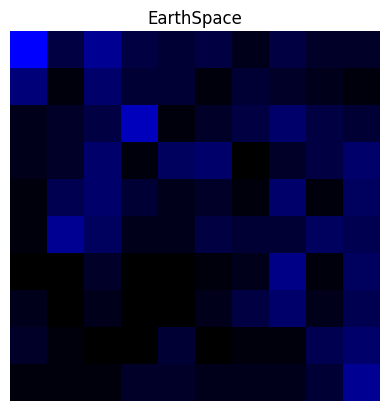
\includegraphics[width=\linewidth]{images/EarthSpace.png}
            \caption{Visualización de EarthSpace}
            \label{fig:EarthSpace}
          \end{subfigure}
          \begin{subfigure}[b]{0.45\textwidth}
            \centering
            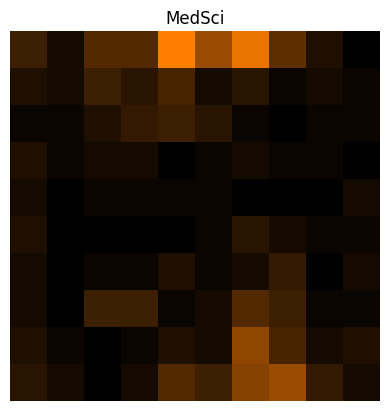
\includegraphics[width=\linewidth]{images/MedSci.png}
            \caption{Visualización de MedSci}
            \label{fig:MedSci}
          \end{subfigure}
          \caption{EarthSpace y MedSci}
          \label{fig:EarthSpaceMedSci}
        \end{figure}

        \newpage

        \begin{longtable}{cccccc}
          \cline{2-6}
                                                                          & \multicolumn{5}{c}{Maquinas de aprendizaje}                                                                             \\ \cline{2-6}
          \endfirsthead
          %
          \endhead
          %
                                                                          & Perceptron                                  & Adeline & \multicolumn{2}{c}{RN con BP} & SVM                             \\ \hline
          \begin{tabular}[c]{@{}c@{}}Tipo de \\ verificacion\end{tabular} & \% de acierto                               & MSE     & MSE                           & \% de aciertos & \% de aciertos \\ \hline
          \begin{tabular}[c]{@{}c@{}}EarthSpace vs\\ MedSci\end{tabular}  & 0.50                                        & 117.68  & 0.47                          & 0.40           & 0.76           \\ \hline
        \end{longtable}

        En base a la visualización de los datos se puede apreciar que la clasificación de las clases EarthSpace y MedSci puede llegar a ser bastante complicada para maquinas de aprendizaje lineales ya que, por medio de la visualización se puede notar que los datos muy probablemente no sean linealmente separables, un hecho que se refleja en el rendimiento del Perceptron y el Adeline, sin embargo maquinas mas complejas logran un mejor resultado al lograr estas crear separaciones no lineales, como se puede puede ver reflejado en el rendimiento de la RN con BP y el SVM, ya que estas ultimas logran un rendimiento mayor que las maquinas de aprendizaje lineales.

  \item LifeSci y Agri

        \begin{figure}[!ht]
          \centering
          \begin{subfigure}[b]{0.45\textwidth}
            \centering
            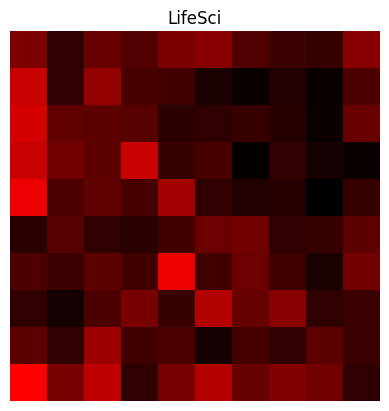
\includegraphics[width=\linewidth]{images/LifeSci.png}
            \caption{Visualización de LifeSci}
            \label{fig:LifeSci}
          \end{subfigure}
          \begin{subfigure}[b]{0.45\textwidth}
            \centering
            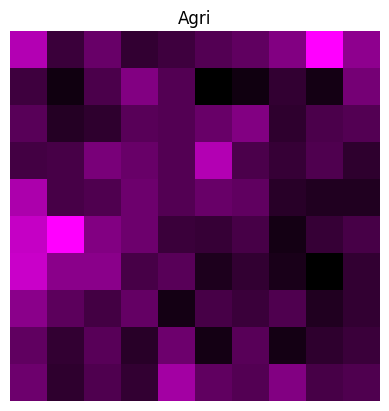
\includegraphics[width=\linewidth]{images/Agri.png}
            \caption{Visualización de Agri}
            \label{fig:Agri}
          \end{subfigure}
          \caption{LifeSci y Agri}
          \label{fig:LifeSciAgri}
        \end{figure}

        \newpage

        \begin{longtable}{cccccc}
          \cline{2-6}
                                                                          & \multicolumn{5}{c}{Maquinas de aprendizaje}                                                                             \\ \cline{2-6}
          \endfirsthead
          %
          \endhead
          %
                                                                          & Perceptron                                  & Adeline & \multicolumn{2}{c}{RN con BP} & SVM                             \\ \hline
          \begin{tabular}[c]{@{}c@{}}Tipo de \\ verificacion\end{tabular} & \% de acierto                               & MSE     & MSE                           & \% de aciertos & \% de aciertos \\ \hline
          \begin{tabular}[c]{@{}c@{}}LifeSci\\ vs Agri\end{tabular}       & 0.54                                        & 1300    & 0.29                          & 0.46           & 0.66           \\ \hline
        \end{longtable}

        En base a la visualización de los datos se puede apreciar que la clasificación de las clases LifeSci y Agri puede llegar a ser bastante complicada para cualquier maquina de aprendizaje ya que, por medio de la visualización se puede notar que los datos se encuentra muy mezclados entre si, evidenciado también por la alta dispersion en la activación de las neuronas del mallado, esta dificultad para aprender a diferencia estas dos clases se ve reflejado en el desempeño de todas las maquinas de aprendizaje dado que ninguna logro clasificaciones significativamente altas en las etapas de verificación, sin embargo las mejores maquinas que logran un mejor desempeño son las RN con BP y el SVM, ya que estas ultimas logran un rendimiento mayor que las maquinas de aprendizaje lineales.

\end{itemize}

\section*{t-SNE}

\subsection*{Descripción de la implementación}

Para la visualización de los datos por medio del algoritmo del t-SNE se utilizo la implementación en python dada por el autor van der Maaten, la cual se puede encontrar en el siguiente enlace \url{https://lvdmaaten.github.io/tsne/}. Para la utilizacion de este algoritmo se realizo un wrapper en el etorno Jupyter Notebook, para cargar los datos y realizar la visualización de los mismos.

Los parametros utilizados para la ejecucion de este algoritmo fueron los siguientes:

\begin{itemize}
  \item Perplexity: 100
  \item Initial dimensions: 35
  \item Iteraciones: 1000
\end{itemize}

\subsection*{Análisis de los resultados}

Se ejecuto el algoritmo con los parámetros mencionados anteriormente para todos los conjuntos de datos, para después graficar el vector de salida del algoritmo en un plano 2D, para poder visualizar los datos de una manera mas sencilla. El obtenido fue el siguiente:

\begin{figure}[!ht]
  \centering
  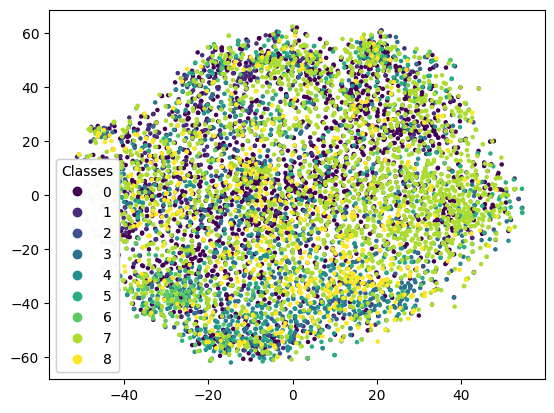
\includegraphics{images/tsne.png}
  \caption{Visualización de los datos por medio del algoritmo t-SNE}
  \label{fig:tsne}
\end{figure}

\newpage

Como se puede observar en la gráfica de la figura \ref{fig:tsne} este algoritmo no logra llegar a una representación visual del conjunto de datos que permita diferenciar las clases de manera clara, esto posiblemente a que el algoritmo t-SNE no es capaz de capturar la estructura de los datos. La gráfica se asemeja mas a una nube de puntos que a un cluster de datos, por lo cual no se puede obtener información relevante de la distribución de los datos.\\

Algunas posibles razones del comportamiento del algoritmo pueden deberse, como lo comenta el autor en su pagina, a una mala entonación del parámetro de perplexity, o a una falta de escalamiento de los datos (normalización o estandarización), sin embargo no se pudieron realizar estas pruebas debido al alto tiempo de ejecución que requiere el algoritmo, para el conjunto de datos utilizado.\\

Como el gráfico no presenta características relevantes o que permitan diferenciar las clases, no es posible realizar un análisis de los resultados obtenidos por las maquina de aprendizaje, ni obtener conclusiones importantes en el comportamiento de las mismas por medio de estas gráfica.

\end{document}